We conduct a set of analyses to understand the factors that contribute to the models' ability to follow instructions, in particular, the effects of  instructions at training and inference (Section~\ref{sec:robustness}), dataset scale (Section~\ref{sec:ablation_datasets}),  model scale (Section~\ref{sec:model_scale}) and carefully-designed negative samples (Section~\ref{sec:negatives}). 
Our analysis in this section focuses on the more powerful \model-full { initialized with T0-3B.  }

\begin{figure}[t!]
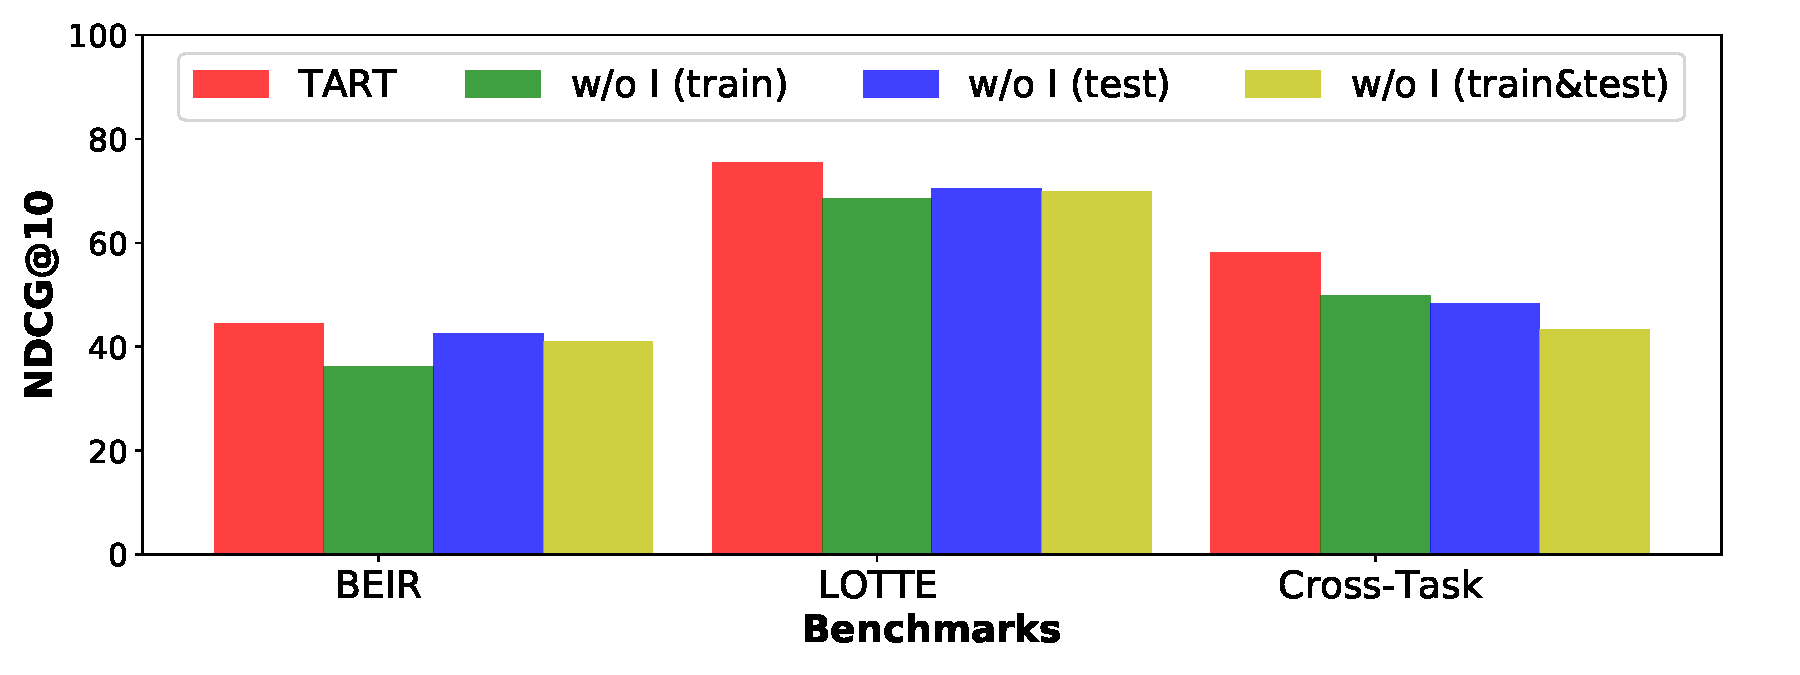
\includegraphics[width=7.5cm]{imgs/instruction_ablations_fixed.pdf}\caption{Ablations of instructions. w/o I (train), w/o I (test), and w/o (train \& test) indicate the ablations (a), (b), and (c), respectively. } \label{fig:inst_effectiveness}
\end{figure}
\begin{figure}[t!]
\centering
\begin{subfigure}[t]{.34\linewidth}
  \centering
  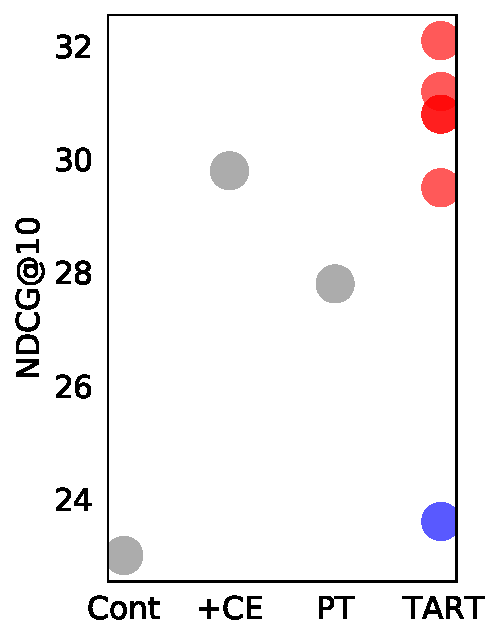
\includegraphics[width=0.98\textwidth,keepaspectratio]{imgs/touche_prompts.pdf}
   \captionsetup{width=0.95\textwidth}
  \caption{Touche-2020}%, pearson correlation = 0.751}
  \label{fig:nfcorpus}
\end{subfigure}%
\begin{subfigure}[t]{.3\linewidth}
  \centering
  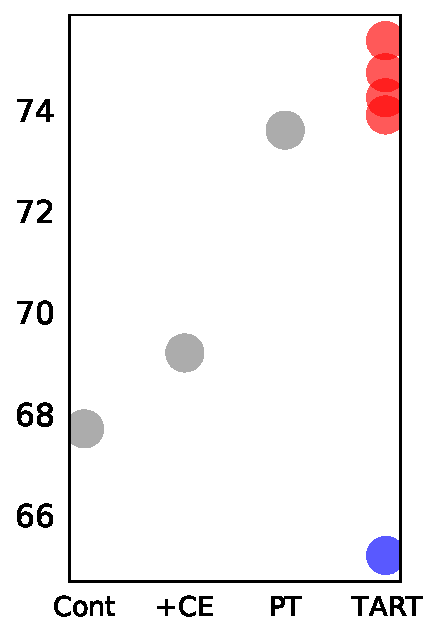
\includegraphics[width=0.98\textwidth,keepaspectratio]{imgs/scifact_prompt.pdf}
   \captionsetup{width=0.95\textwidth}
  \caption{SciFact}%, pearson correlation = 0.751}
  \label{fig:scifact}
\end{subfigure}%
\begin{subfigure}[t]{.3\linewidth}
  \centering
  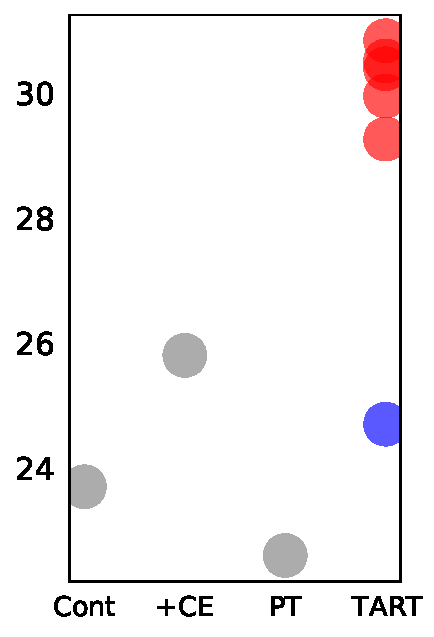
\includegraphics[width=0.98\textwidth,keepaspectratio]{imgs/climate_fever.pdf} 
  \captionsetup{width=0.95\textwidth}
  \caption{C-FEVER}%, pearson correlation = 0.785}
  \label{fig:arguana}
\end{subfigure}%
\caption{Performance variance across different instructions. {C-Fever indicates Climate-Fever.} Blue circles indicate performance without instructions at test time, while red circles indicate performance with different instructions. 
% performance with irrelevant or vague instructions. 
``PT'', ``Cont'', ``+CE'' denote Promptagator, Contriever and Contriever+CE.  }
\label{fig:prompt_variance}
\end{figure}
\subsection{Effects of Instructions}
\label{sec:robustness}
\paragraph{Ablating instructions.} 
To analyze the effectiveness of instructions, we compare \model-cross with three variants: (a) {\it train without instructions, test with instructions} prepends instructions at test time only to test if the models just exploit keyword matching only at test time; (b) {\it train with instructions, test without instructions} uses \model-full without instructions at test time; (c) {\it train without instructions, test without instructions} does not use instructions at all during training and test time. 

Figure~\ref{fig:inst_effectiveness} shows the performance of those baselines. 
On all benchmarks, ablating instructions during training or test time causes a notable performance drop. 
We also see that a model trained with instructions but given no instruction at test time still yields a few performance improvements over the model trained completely without instructions, indicating the effectiveness of incorporating instructions during multi-task training. 

\paragraph{Robustness toward instructions.}
We evaluate \model-full's robustness towards diverse instructions. 
Figure~\ref{fig:prompt_variance} shows the performance variance given multiple different instructions. 
The blue circles represent the performance with no instruction.
Instructions significantly improve model performance without instructions. Although different instructions give small performance variance, \model-full often outperforms other competitive baselines when informative and correct instructions are given.
We also observe larger performance deterioration when inaccurate instructions are given. 
See Table~\ref{tab:prompt_performance_full_list} for individual instructions and performance.

 \begin{figure}[t!]
\centering
\begin{subfigure}[t]{.46\linewidth}
  \centering
  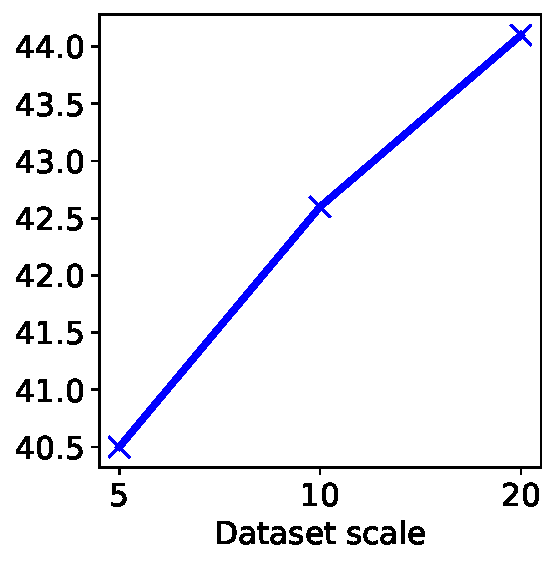
\includegraphics[width=0.9\textwidth,keepaspectratio]{imgs/dataset_scale.pdf}
  \captionsetup{width=0.95\textwidth}
  \caption{Dataset scale}
  \label{fig:dataset_scale}
\end{subfigure}%
\begin{subfigure}[t]{.52\linewidth}
  \centering
  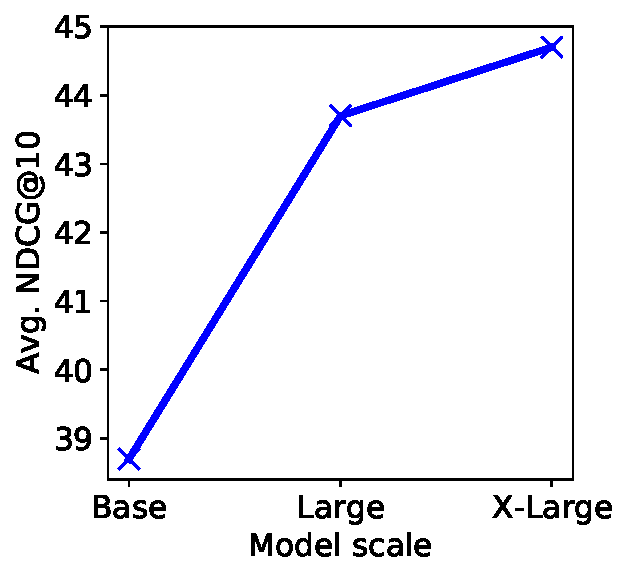
\includegraphics[width=0.9\textwidth,keepaspectratio]{imgs/model_scale.pdf}
  \captionsetup{width=0.95\textwidth}
  \caption{Model scale}
  \label{fig:model_scale}
\end{subfigure}%
\caption{Analysis of dataset and model scale. 
}
\label{fig:analysis}
\end{figure}


\subsection{Dataset Scale}
\label{sec:ablation_datasets}
To assess the effectiveness of diverse datasets, we conduct dataset ablation experiments, where we ablate datasets during training. 
Following prior work on language models instruction tuning, we conduct these experiments based on the number of datasets~\cite{wang2022benchmarking} and task clusters~\cite{wei2022finetuned}.  In addition, we run ablations based on the number of domains, where we ablate datasets based on their source domains. 
Figures~\ref{fig:dataset_scale} and \ref{fig:ablation_data} show these experiments' results. 

\paragraph{Number of datasets.}
Figure~\ref{fig:dataset_scale} shows the average performance on four BEIR datasets of \model-full trained on randomly sampled 5, 10 and 20 datasets. 
We observe that increasing the number of the training datasets helps \model to perform better. 
% In addition to domain and task diversity, the diversity of instructions observed during training may also improve performance.


\paragraph{Task diversity.}
As shown in Figure~\ref{fig:ablation_data}, task diversity is a key to improve models' zero-shot transfer performance. 
QA only struggles on Arguana, where the tasks significantly differ from QA. 


\paragraph{Domain diversity.}
Figure~\ref{fig:ablation_data} shows that having more diversity in training datasets' domains is also crucial, especially when the target datasets are in non-general domains. For instance, a model trained only on Wikipedia datasets struggles on Touche-2020 or SciFact, where documents come from argument websites and scientific papers, respectively. 

\begin{figure}[t!]
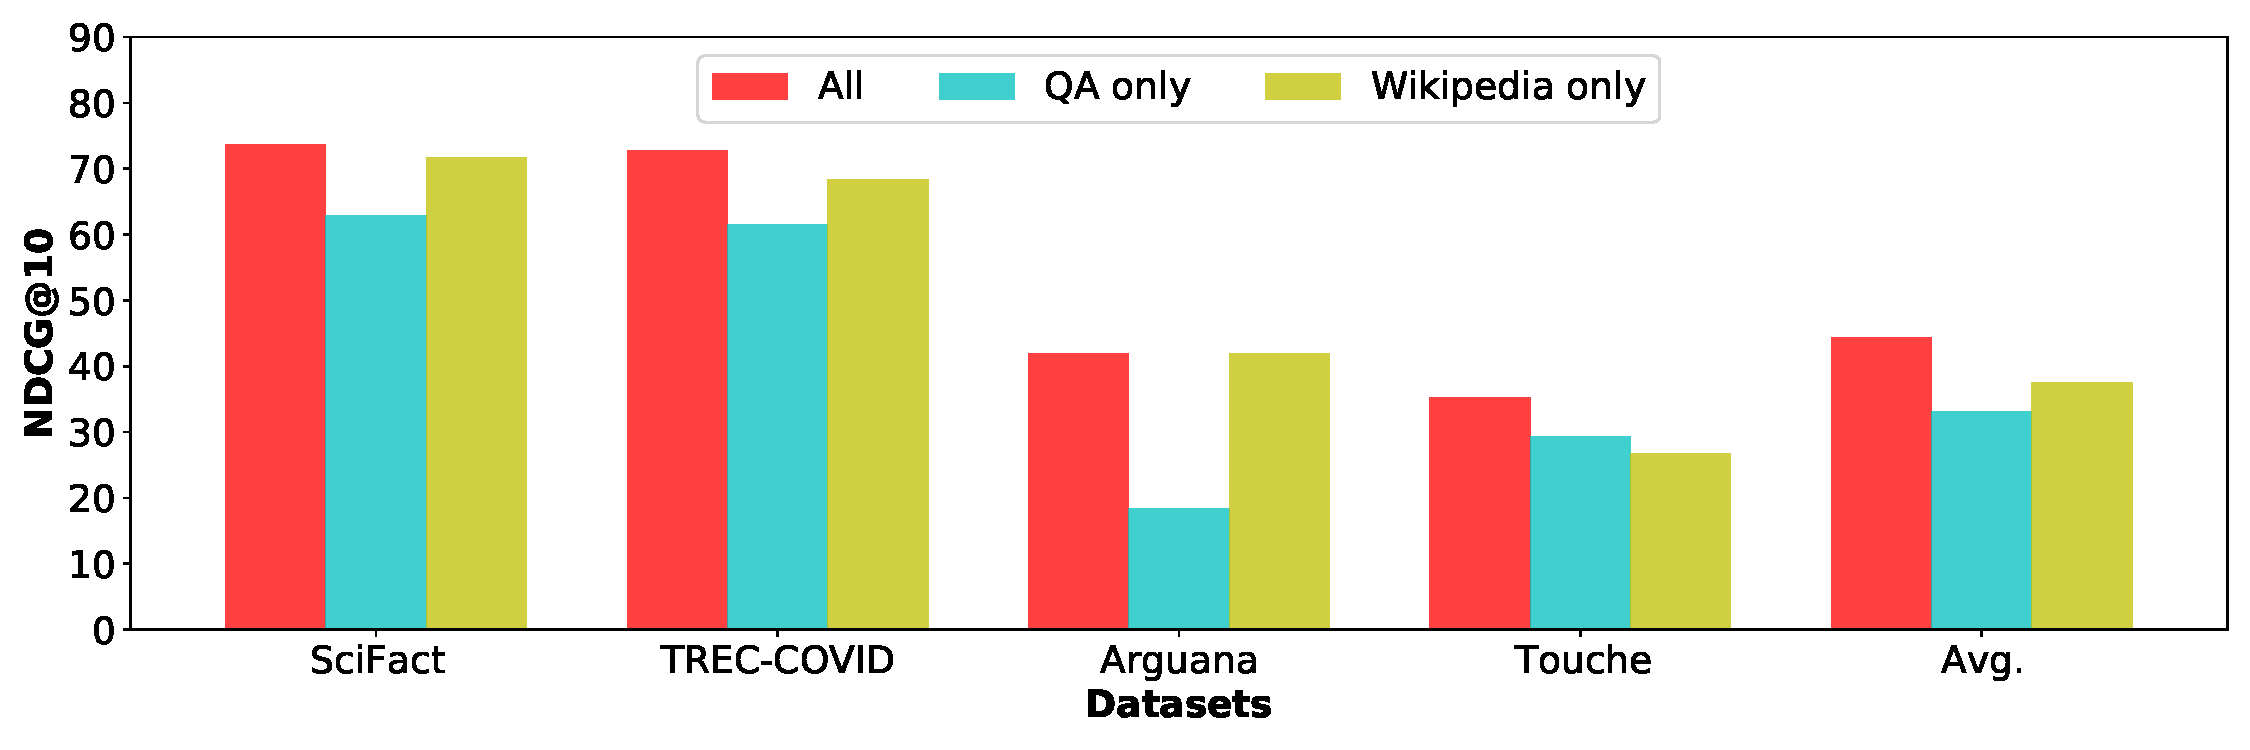
\includegraphics[width=8cm]{imgs/domain_ablations.pdf}\caption{Dataset ablation results. Wikipedia-only denotes \model-full performance trained on Wikipedia-based datasets only. QA-only denotes the model trained on QA datasets only. 
% Even with the same query, the outputs are different.  
} \label{fig:ablation_data}
\end{figure}

\subsection{Model Scale}
\label{sec:model_scale}
We test different \model-full sizes to see how model scale affects final performance. 
Prior work has shown that scaling up re-ranking models often improves reranking performance~\cite{rosa2022no}, and models' instruction-following abilities improve as models get larger~\cite{wang2022benchmarking,sanh2022multitask,wei2022emergent}.
We investigate how model scale affects the ability to generalize to new tasks {\it and} follow instructions. 
For a fair comparison, we train \model-full using different T5 LM-Adapt (base, large, and XL) and evaluate performance using them to rerank the top 100 Contriever results. 

Figure~\ref{fig:model_scale} shows \model-full's average performance across different model scales.  
We observe clear performance improvements by increasing model size as observed in prior work on LLM. 

\begin{figure}[t!]
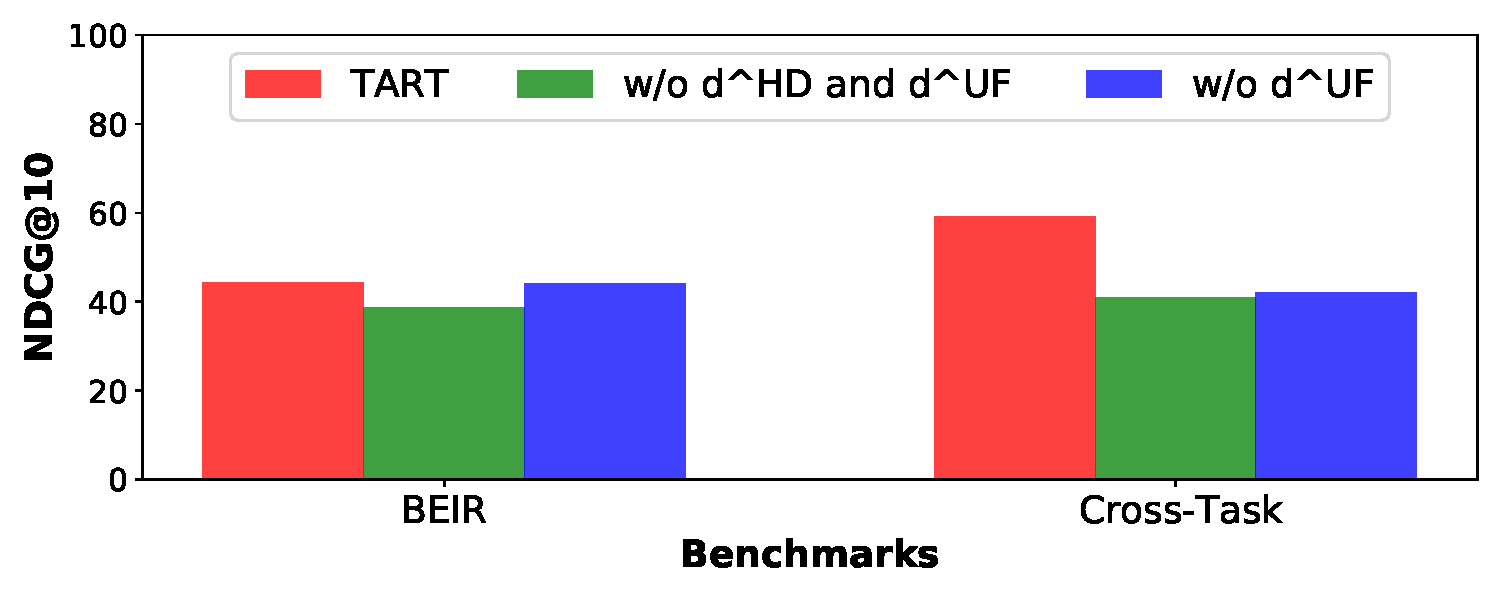
\includegraphics[width=8cm]{imgs/negative_sample_ablations.pdf}\caption{{Ablations of negative samples. 
``w/o $\boldsymbol{d}^{\rm HD}$ and $\boldsymbol{d}^{\rm UF}$'' denotes a model trained without hard and instruction-unfollowing negative documents while ``w/o $\boldsymbol{d}^{\rm UF}$''  ablates instruction-unfollowing documents only. }
% Even with the same query, the outputs are different.  
} \label{fig:negative_ablations}
\end{figure}
\subsection{Negative Samples}
\label{sec:negatives}
{
We analyze the effectiveness of negative samples by ablating them during training. 
Figure~\ref{fig:negative_ablations} shows the performance of the models trained without negative samples on BEIR and \task. 
Adding more challenging negative documents (i.e.,  $\boldsymbol{d}^{\rm HD}$ and $\boldsymbol{d}^{\rm UF}$) during training largely improves the model performance on BEIR.
Moreover, the model trained without instruction-following samples (w/o $\boldsymbol{d}^{\rm UF}$) results in lower \task performance, although this model performs on par with the original \model-full on BEIR. 
This indicates that our new instruction-unfollowing negative documents largely contribute to improving the ability to distinguish instructions and are thus crucial to build a robust task-aware retrieval system. 
}


